\setlength{\parindent}{2ex}
\begin{chapter}{Numerical Results}\label{chapter:results}

%\section{}
Finally, we implement the preceding development on synthetically derived data as well as on calibration radiographs from a high energy X-ray imaging system.
The synthetic data is generated by adding simulated independent and identically distributed Gaussian measurement noise to the forward image of a PSF with a known analytic form.
The radiographic data comes from a large-scale diagnostic imaging system at the U.S. Department of Energy's Nevada National Security Site.
In both cases, the theoretically predicted deficiency in the $\delta$-chain is demonstrated using the statistical diagnostics introduced at the end of \Cref{chapter:mcmctheory} in \Cref{sec:evaluatingConvergence}.
The standard Gibbs sampler is compared to both versions of the partially collapsed Gibbs sampler derived in \Cref{chapter:computational}, and we investigate the trade-off between chain convergence and computational complexity in terms of number of expensive matrix factorizations.
We demonstrate that even with taking into account the reduced computational complexity of the standard Gibbs sampler, partially collapsing $\vect p$ in the $\delta$ component improves convergence of the joint Markov chain.

\section{Synthetic PSF Reconstruction}
To simulate synthetic data, we reconstruct a radial profile of a two-dimensional Gaussian kernel
\begin{equation} \label{eq:syntheticx}
  p(r) = (2\pi\sigma^2)^{-1} e^{\frac{-r^2}{2\sigma^2}},
\end{equation}
where $\sigma = \frac1{15}$ is chosen so that the effective width of the kernel is about 20\% of the image width when scaled to $[-1,1]$.
Observe that in the case of a two-dimensional Gaussian, the action of the forward operator in \eqref{eq:radialForwardModelDeterministic} is the scaled error function
\begin{equation} \label{eq:syntheticb}
  b(s) = \frac 1{\sqrt{2\pi}\sigma} \int_{-\infty}^s e^{-\frac{s'^2}{2\sigma^2}}\,ds'.
\end{equation}
We synthetically add measurement error with noise strength that is 2\% of the strength of the signal.
For the PCG algorithms, the inner Metropolis-Hastings step was computed with $n_{mh} = 1$ and $n_{mh} = 5$, and the initial values of $\lambda_0 = 1$ and $\delta_0 = 1$ were used for each implementation.
\begin{figure}[p]
  \begin{center}
  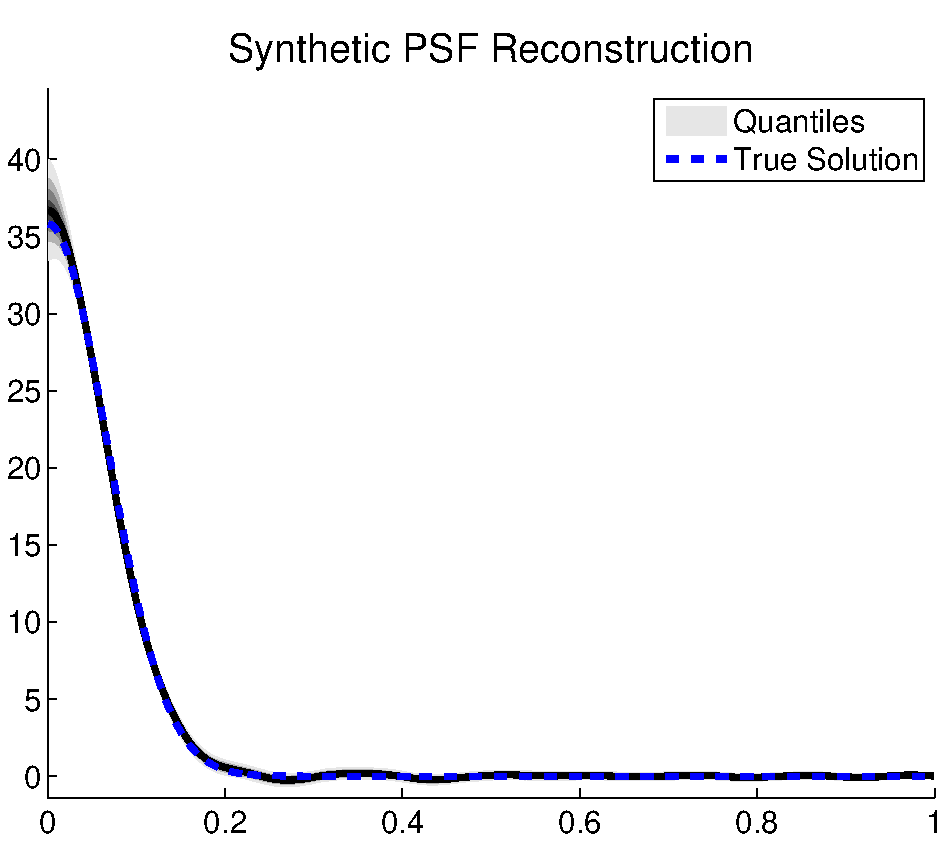
\includegraphics[width=.4\textwidth]{figures/syntheticPSFrecon.pdf}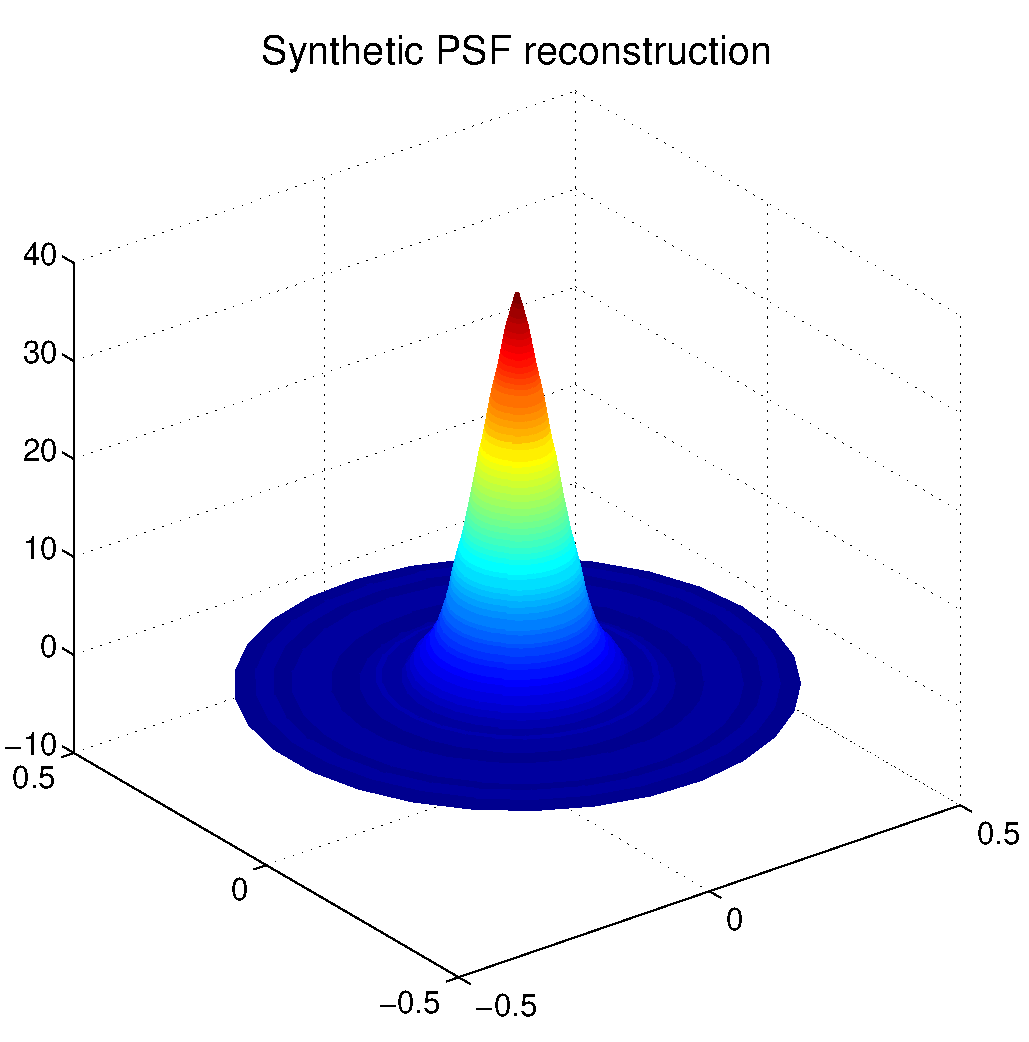
\includegraphics[width=.4\textwidth]{figures/synthetic2dPSFrecon.pdf}
  \caption{The 10\%, 25\%, 50\%, 70\%, and 90\% quantiles of the reconstructed 1D radial representations of the synthetic Gaussian PSF (left) along with the mean 2D reconstruction (right).} \label{fig:syntheticPsfRecon}
  \end{center}
\end{figure}
\begin{figure}[p]
\begin{center}
  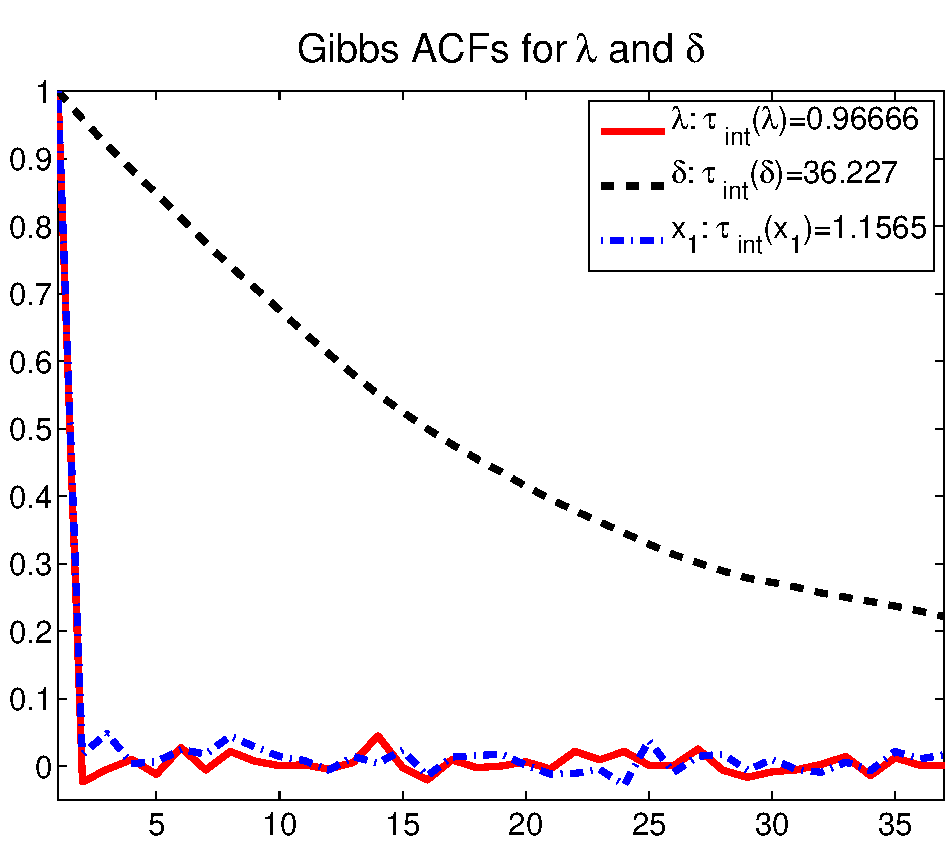
\includegraphics[width=.35\textwidth]{figures/ACFlambdelPSFreconGibbsM1.pdf}  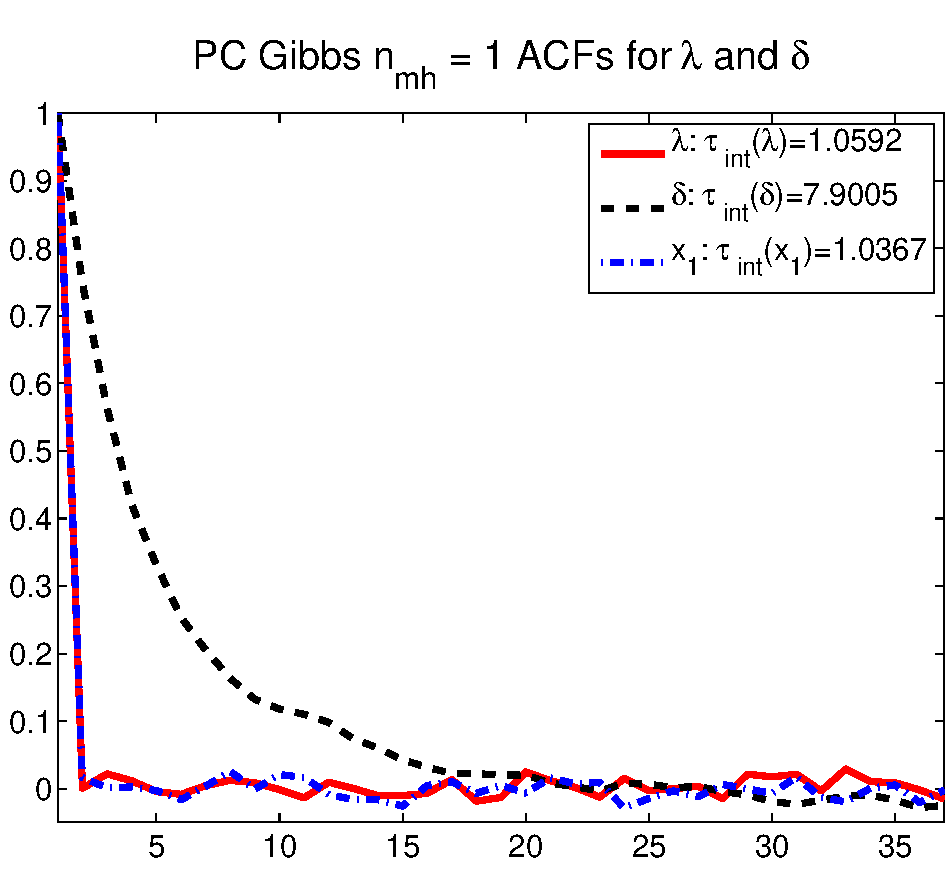
\includegraphics[width=.35\textwidth]{figures/ACFlambdelPSFreconPCGibbsM1.pdf}\\\vspace{2em}
  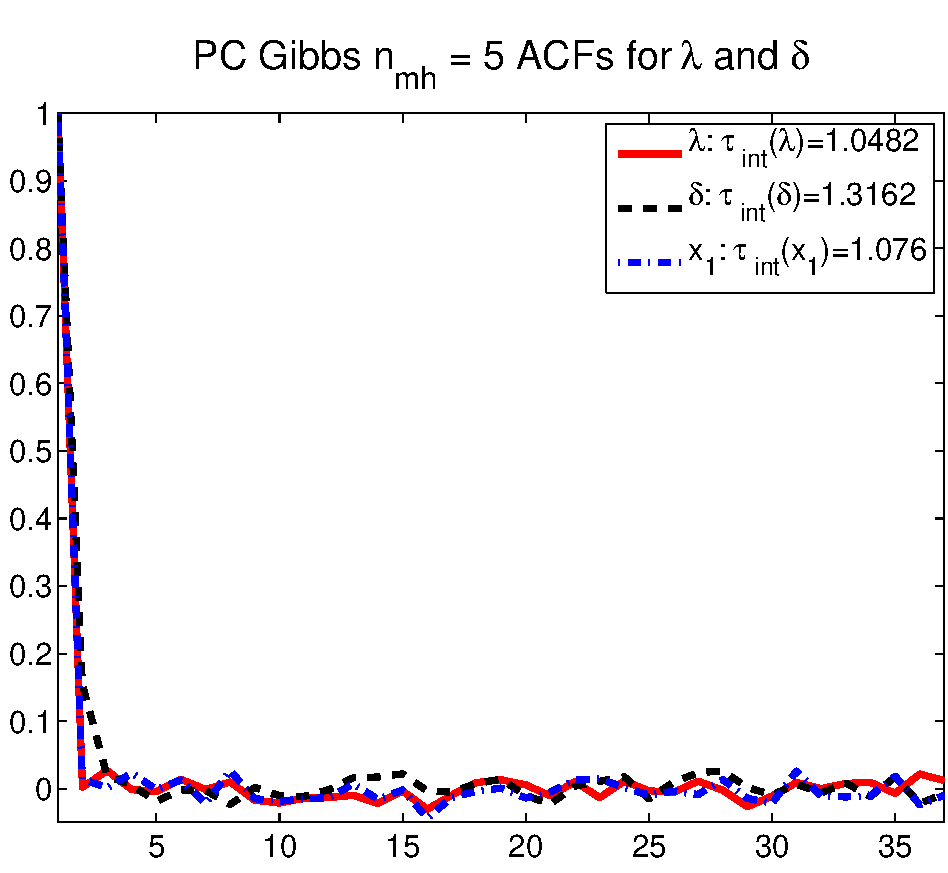
\includegraphics[width=.35\textwidth]{figures/ACFlambdelPSFreconPCGibbsM5.pdf}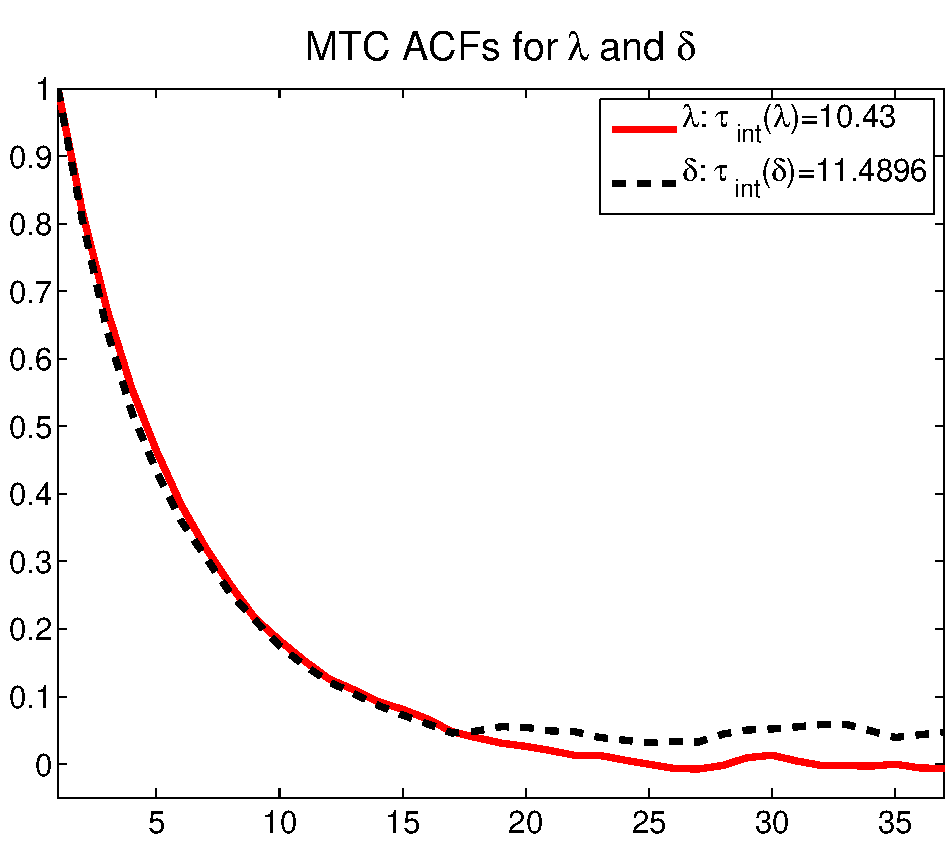
\includegraphics[width=.35\textwidth]{figures/ACFlambdelPSFreconMTC.pdf}
\end{center}
\caption{Autocorrelation plots for PSF reconstruction for synthetic data of the chains $\lambda$, $\delta$ and the central discretization point of $\vect p$: in the upper-left are the ACF for MCMC chains of $\lambda$, $\delta$ and central pixel of the radial profile for the Gibbs sampler; on the upper-right are the plots for the PC Gibbs sampler with 1 inner MH step; on the lower-left are plots for the PC Gibbs sampler with 5 inner MH steps; and in the lower-right are plots for the MTC sampler.} \label{fig:syntheticPsfACF}
\end{figure}

The computed mean of the posterior density is shown in \Cref{fig:syntheticPsfRecon} (right) in 2D, along with quantiles of the radial representations (left). 
The true solution is also shown on the left, showing the accuracy of the reconstruction.  
Note that the most uncertain region of the reconstruction are the initial discretization points corresponding to the height of the PSF, however, the true solution falls within the 90\% quantiles at each point.

The MCMC diagnostics are summarized in Table \Cref{tab:PSFDeltaChain}. 
With the exception of the $\delta$ chain generated by the Gibbs sampler, each method yields Geweke $p$-values sufficiently large to indicate strong statistical evidence that burn-in has completed. 
The lack of convergence for the Gibbs sampler $\delta$ chain is the likely cause for the mean estimate of $\delta$ being marginally larger than the other three. 
The large autocorrelation in the $\delta$ chain generated by the Gibbs sampler results in an ESS that is significantly lower than the other three algorithms. 
Using \#Chol/ESS as an effeciency measure, we see that PC Gibbs with $n_{mh}=5$ is the most effecient of the four methods.
\begin{table}[h]
\begin{center}
  \begin{tabular}{l|ccccccc}
    \hline
% Jan. 9 values initial delta = 1 and initial lambda = 1
    Algorithm       & $\hat{\lambda}_{\rm MCMC}$& $\hat{\delta}_{\rm MCMC}$  & $\lambda$-$p_{\rm Geweke}$&$\delta$-$p_{\rm Geweke}$& IACT & ESS    & \#Chol/ESS \\
     & $(\times 10^{4})$ & ($\times 10^{-8}$) & & \\
    \hline
	      Gibbs &                 1.102 &                 6.132 &                    0.998 &                    0.850& 36.2 &  138.0 &      72.4 \\
PC Gibbs &                 1.102 &                 5.611 &                    0.992 &                    0.943&  7.9 &  633.0 &      31.6 \\
\hspace{.2in} $n_{mh}= 1$ & & & & & & & \\
PC Gibbs &                 1.102 &                 5.515&                    0.999 &                    0.985&  1.3 & 3799.6 &      15.8 \\
\hspace{.2in} $n_{mh}= 5$ & & & & & & & \\
		MTC &                 1.099 &                 5.419 &                    0.998 &                    0.934& 11.5 &  473.2 &      21.1 \\
    % Dec. 11 values initial delta = norm(B) and initial lambda = 1/var( b(1:10) )
%    Gibbs             &                   0.997 &                    0.850& 46.3 &  107.9 &      92.6 \\
%    PC Gibbs $m_h=1$  &                   0.999 &                    0.955&  5.2 &  954.6 &      21.0 \\
%    PC Gibbs $m_h=5$  &                   0.998 &                    0.981&  1.7 & 2981.8 &      20.1 \\
%    MTC               &                   0.990 &                    0.950& 11.3 &  443.3 &      22.6 \\
    \hline
  \end{tabular}
  \caption{ Statistical diagnostics for the $\lambda$ and $\delta$ chains associated with the synthetic PSF reconstruction problem. The total chain length is $M=10^4$, with a burn-in of $k_{\rm burnin} = 5\times10^3$. The first column are the post-burn-in chain means of $\lambda$ and $\delta$. The maximum IACT of $\lambda$ and $\delta$ are used to calculate IACT and ESS. For MTC algorithm, $\lceil(M-k_{\rm burnin})/\tau_{\rm int}\rceil$ is added to \#Chol to evaluate the efficiency.} \label{tab:PSFDeltaChain}
\end{center}
\end{table}

The chain autocorrelation plots in \Cref{fig:syntheticPsfACF} give additional insights. 
First, for the Gibbs sampler, the autocorrelation of the $\delta$ chain is quite large, and the $\lambda$ chain is approximately uncorrelated, as values in Table \Cref{tab:PSFDeltaChain} suggested would be the case. 
Note also that sampling jointly in the MTC algorithm degrades the efficiency of $\lambda$. 
Finally, note that we also include autocorrelation plots for the first component, $x_1$, of $\vect p$, in order to show that the $\vect p$ chain is essentially uncorrelated, and hence that the correlation in the MCMC chains generated by Gibbs and PC-Gibbs samplers is driven by the $\delta$ chain. 

\section{PSF reconstruction from X-ray Radiographs}\label{subsec:real data}

%We now carry out the analysis outlined above on a synthetic example and on actual data from an X-ray radiographic imaging system at the U.S.~Department of Energy's research complex at the Nevada National Security Site (NNSS) operated by National Security Technologies LLC.

Next we reconstruct the point spread function of a high energy X-ray imaging system at the U.S. Department of Energy's Nevada National Security Site. The real edge data is shown in \Cref{fig:CygnusPsfRecon} (upper left) along with a horizontal cross-section across the edge (upper right). The mean MCMC reconstruction is shown in \Cref{fig:CygnusPsfRecon} (lower left), along with the 10\%, 25\%, 50\%, 70\%, and 90\% quantiles of the chain $\bm{x}^{k}$.
We estimated the PSF at grid points using the chain-wise mean after burn-in, $\hat {\vect p} = \frac 2M \sum_{k=M/2+1}^M {\vect p}^{k}$.
Since the true PSF is unknown, we evaluate the accuracy of the estimation by its discrepancy; i.e. we compared forward mapping of the estimate $\Ab {\hat{\vect p}}$ with the given data $\bm b$.  This is shown in both linear and logarithmic scales in \Cref{fig:CygnusPsfRecon} (lower right). 
In both cases the discrepancy is quite low, except at very low intensities where the data is dominated by the noise, which can be seen in the logarithmic scale.
 %The true solution is not known and is thus not plotted along with the reconstructions.

\begin{figure}[h]
  \begin{center}
  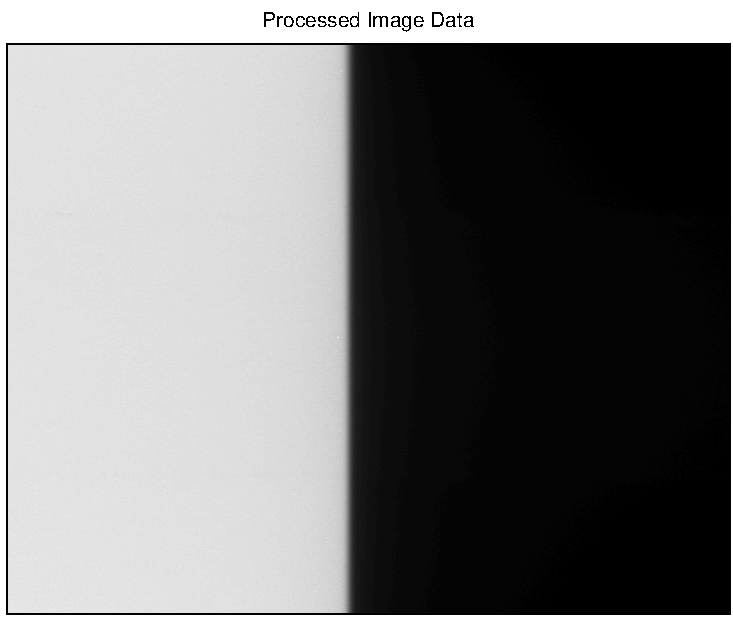
\includegraphics[height=2in]{figures/cygnusImage.pdf}\hspace{2em}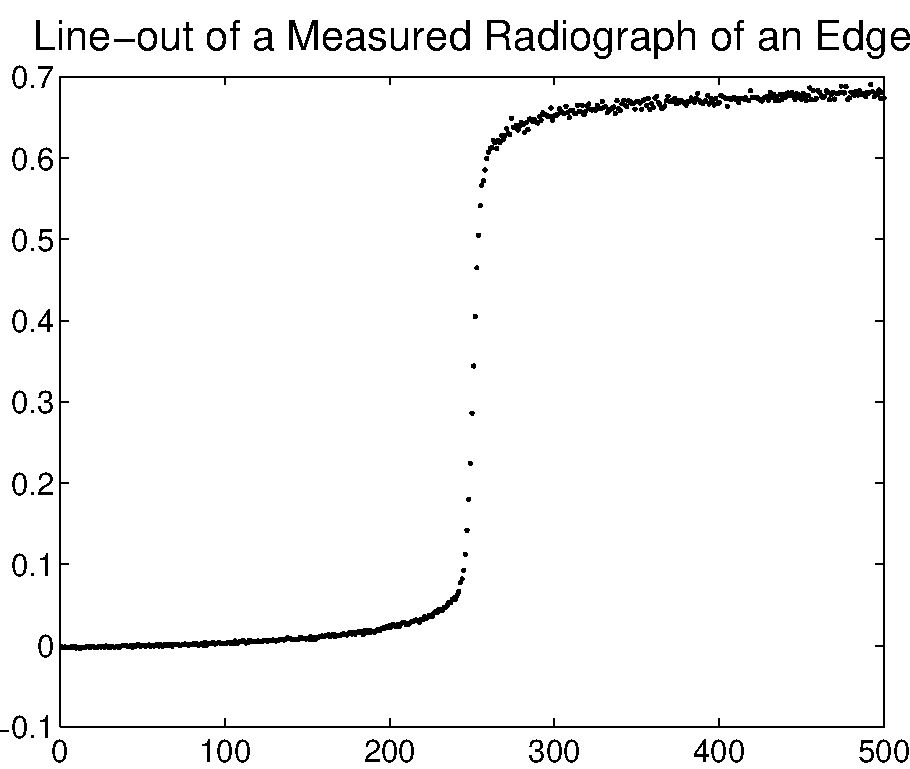
\includegraphics[height=2in]{figures/cygnusLineout.pdf}\\\vspace{2em}
  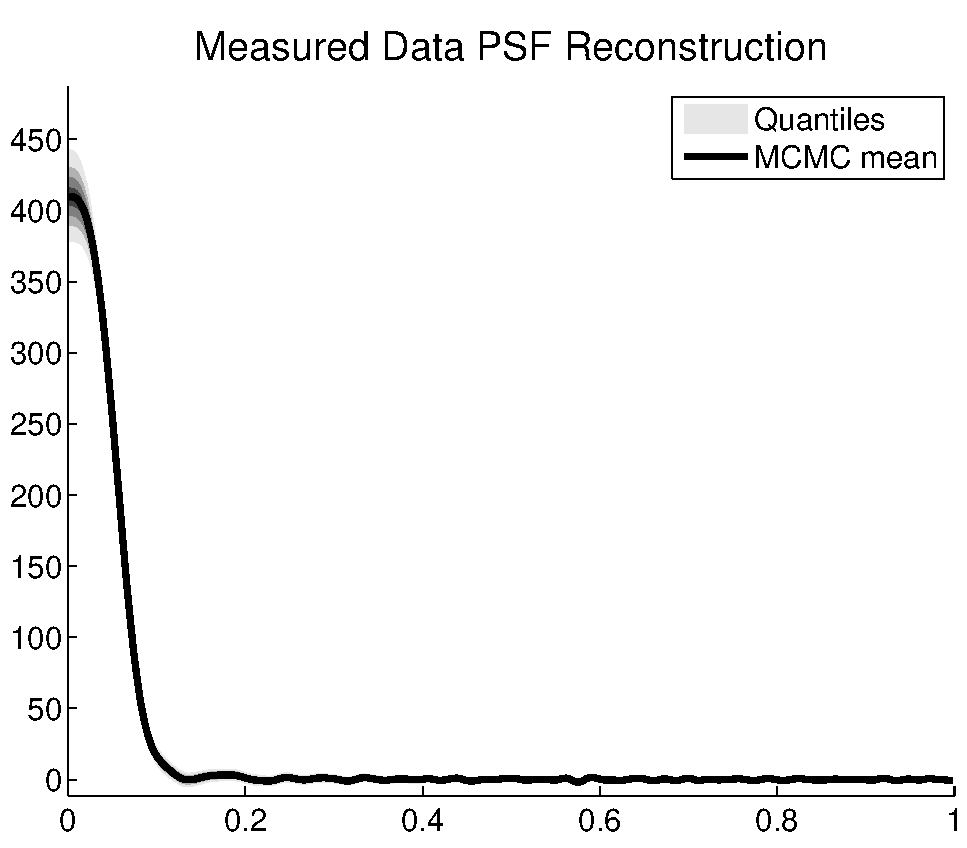
\includegraphics[height=2in]{figures/cygnusPSFrecon.pdf}\hspace{2em}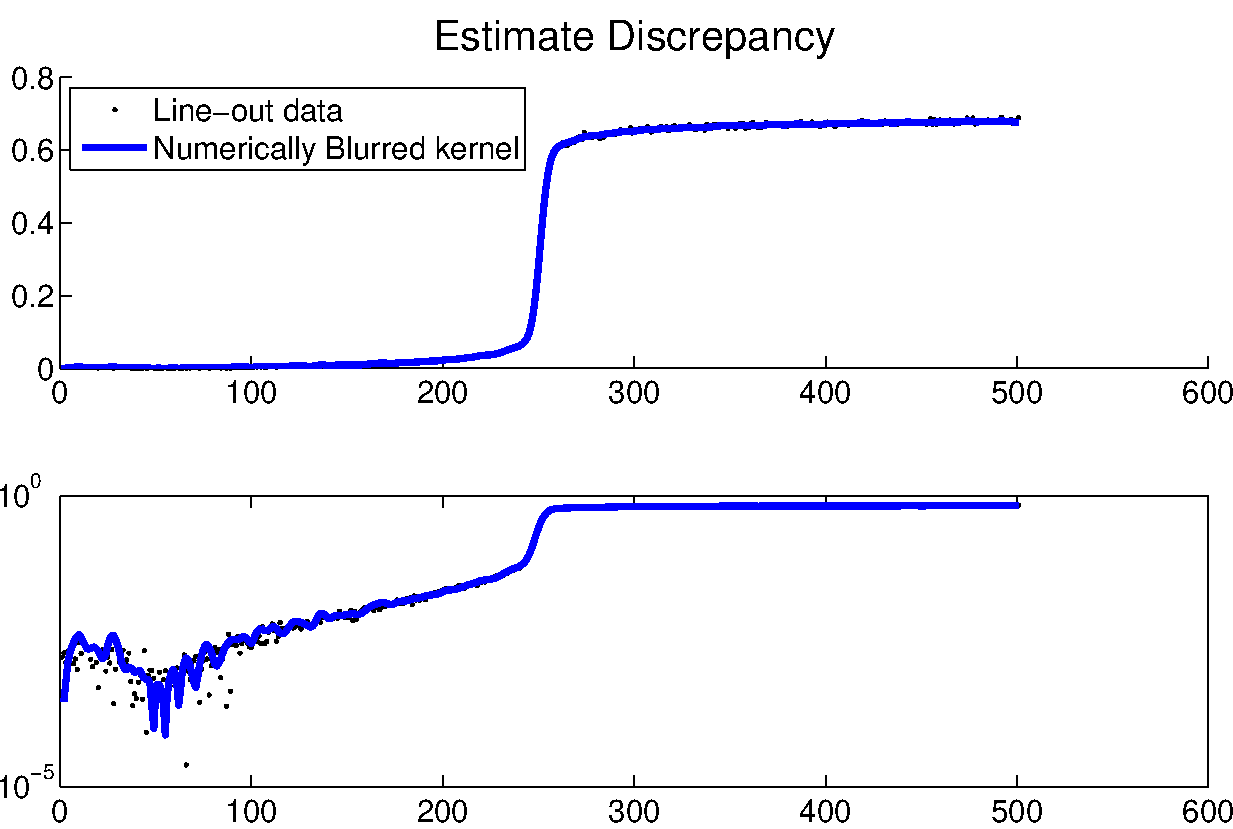
\includegraphics[height=2in]{figures/discrepencyPSF.pdf}
  \caption{
  PSF reconstructions for radiographic data: in the upper left corner are the radiographic image data;
  in the upper right corner is a line-out taken from the image data;
  in the lower left corner are the central 10\%, 25\%, 50\%, 70\%, and 90\% quantiles of the posterior reconstruction of $\bm x$ for each pixel;
  in the lower right corner are plots of the forward mapped discrepancy of the post burn-in chain mean.
  } \label{fig:CygnusPsfRecon}
  \end{center}
\end{figure}

As with the synthetic data, the PC-Gibbs algorithm with $n_{mh}=5$ results in the largest ESS and the most efficient chain (as measured by $\#$Chol/ESS).

\begin{table}[h]
\begin{center}
  \begin{tabular}{l|ccccccc}
    \hline
    Algorithm           & $\hat{\lambda}_{\rm MCMC}$& $\hat{\delta}_{\rm MCMC}$& $\lambda$-$p_{\rm Geweke}$&$\delta$-$p_{\rm Geweke}$& IACT & ESS    & \#Chol/ESS \\
     & $(\times 10^{4})$ & ($\times 10^{-10}$) & & \\
    \hline
	          Gibbs &                 9.146 &               1.245  &                     0.995 &                    0.964& 14.0 &  357.6 &      28.0 \\
PC Gibbs  &                 9.167 &               1.191  &                     0.995 &                    0.998&  8.5 &  587.3 &      34.1 \\
 \hspace{.2in}$n_{mh}=1$ & & & & & & & \\
PC Gibbs &                 9.178 &               1.189  &                     0.994 &                    0.980&  1.5 & 3278.5 &      18.3 \\
\hspace{.2in} $n_{mh}=5$ & & & & & & & \\
		    MTC &                 9.090 &               1.200  &                     0.996 &                    0.969& 12.5 &  432.2 &      23.1 \\
    \hline
  \end{tabular}
  \caption{ Statistical diagnostics for the $\lambda$ and $\delta$ chains associated with the measured data PSF reconstruction problem. The total chain length is $M=10^4$, with a burn-in of $k_{\rm burnin} = 5\times10^3$. The first column are the post-burn-in chain means of $\lambda$ and $\delta$. The maximum IACT of $\lambda$ and $\delta$ are used to calculate IACT and ESS. For MTC algorithm, $\lceil(M-k_{\rm burnin})/\tau_{\rm int}\rceil$ is added to \#Chol to evaluate the efficiency.} \label{tab:CygnusPsfRecon}
\end{center}
\end{table}

\begin{figure}[h]
\begin{center}
  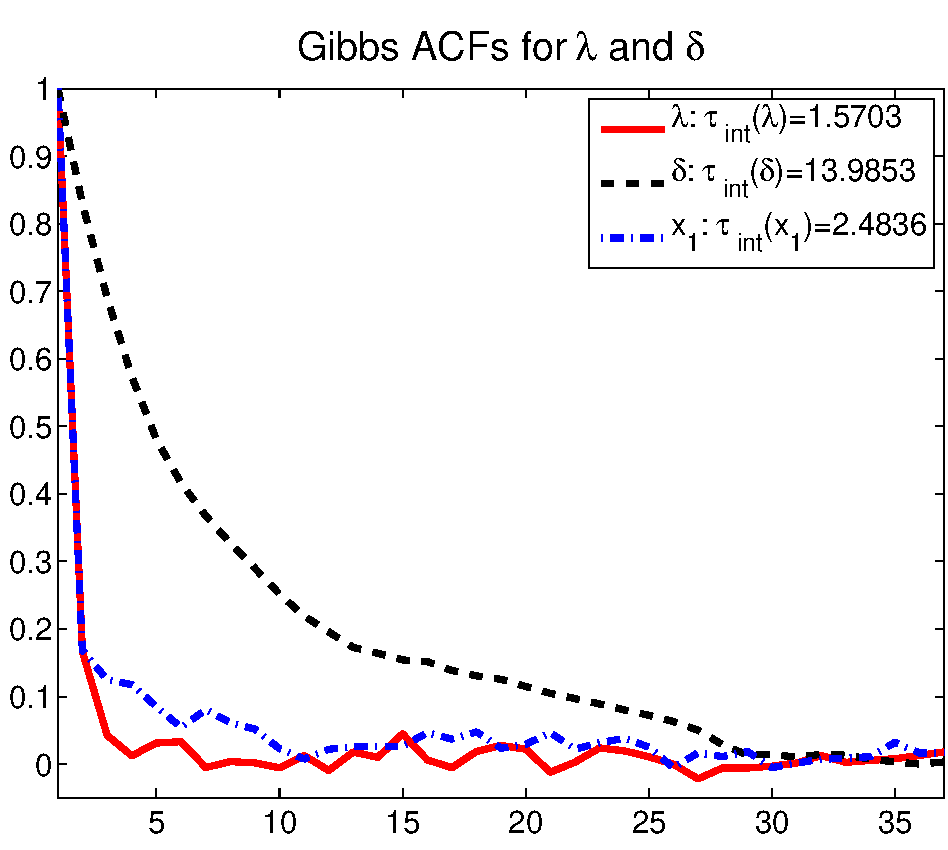
\includegraphics[width=.35\textwidth]{figures/CygnusACFlambdelPSFreconGibbsM1.pdf}  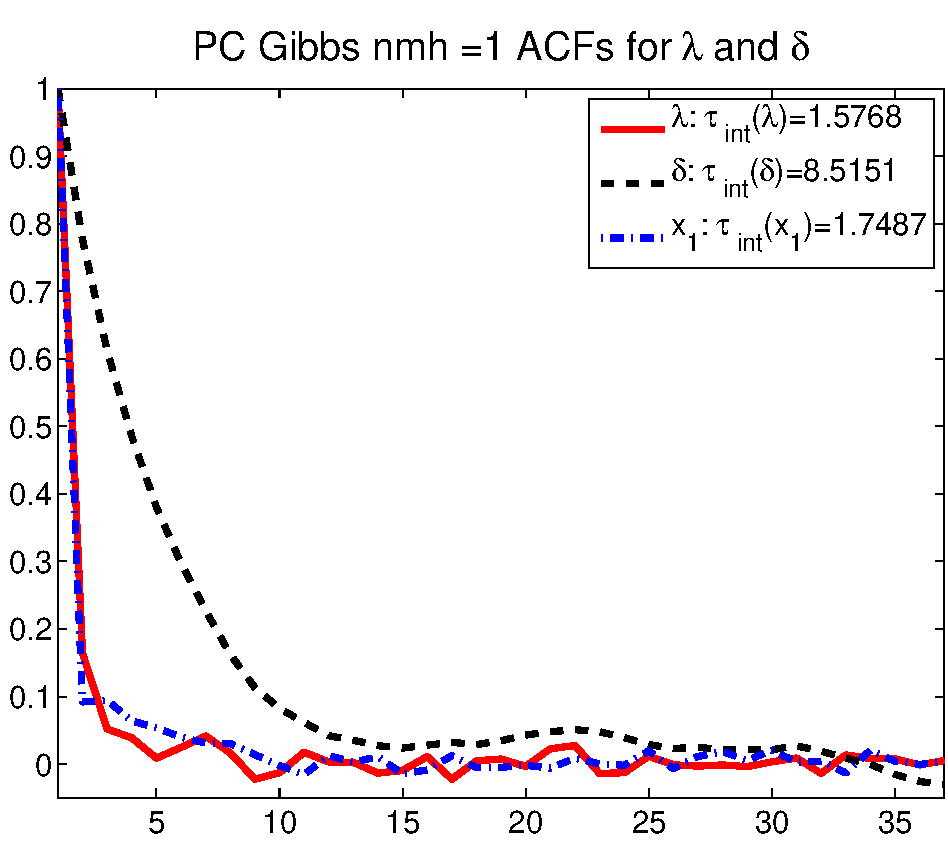
\includegraphics[width=.35\textwidth]{figures/CygnusACFlambdelPSFreconPCGibbsM1.pdf}\\\vspace{2em}
  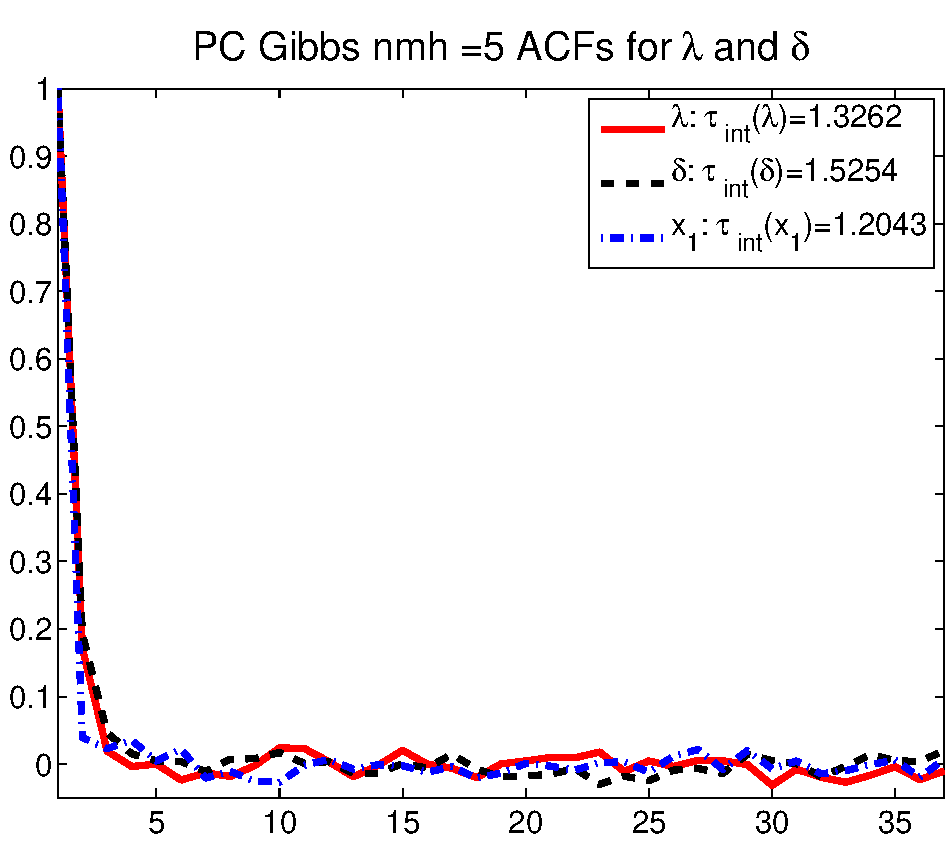
\includegraphics[width=.35\textwidth]{figures/CygnusACFlambdelPSFreconPCGibbsM5.pdf}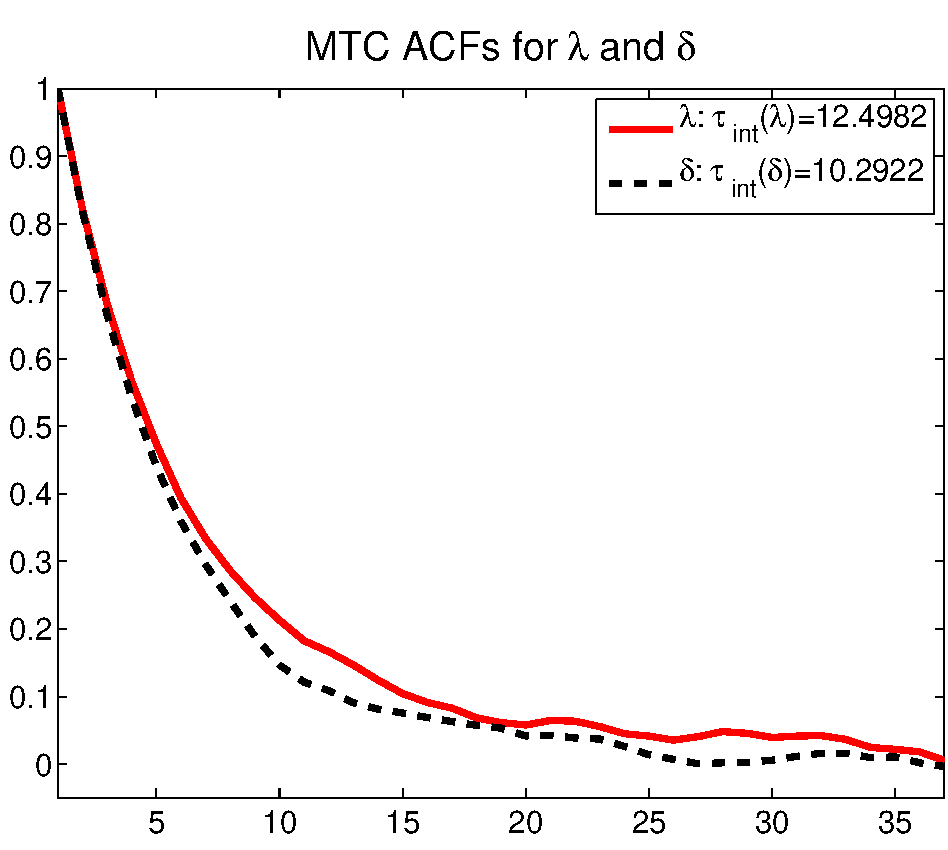
\includegraphics[width=.35\textwidth]{figures/CygnusACFlambdelPSFreconMTC.pdf}
\end{center}
\caption{Autocorrelation plots for PSF reconstruction for the measured data of $\lambda$ and $\delta$ chains: in the upper-left are the ACF for MCMC chains of $\lambda$, $\delta$ and central pixel of the radial profile for the Gibbs sampler; on the upper-right are the plots for the PC Gibbs sampler with 1 inner MH step; on the lower-left are plots for the PC Gibbs sampler with 5 inner MH steps; and in the lower-right are plots for the MTC sampler.} \label{fig:psfACF}
\end{figure}

\section{Conclusions} \label{sec:Conclusions}

\begin{com}
Our focus in this paper is two fold. 
First, we address the degeneracy issue pointed out in \cite{AgaBarPapStu} for the Gibbs sampler above when it is applied to linear inverse problems. 
Specifically, the main theoretical result in \cite{AgaBarPapStu} shows that as the numerical mesh size tends to zero, the autocorrelation of the $\delta$ chain increases, to the extent that in the infinite limit, the MCMC chain will stay fixed on the initial value $\delta_0$. 
The result is that for problems with a fine mesh, the $\delta$ chain is highly correlated and hence a huge number of samples are needed. 
We overcome this by applying the partially collapsed Gibbs framework to the Gibbs sampler, yielding two related MCMC methods, neither of which have have the $\delta$ chain correlation issues. 
Second, our paper focuses on the application of PSF reconstruction in X-ray imaging, which to our knowledge has not appeared elsewhere in the inverse problems literature. 
To that end, we present details for what we believe is a novel derivation of the inverse problem, which makes use of radial symmetry and a square-Laplacian regularization (or precision) matrix. 
Finally, we test our MCMC methods on this inverse problem, using both a synthetic test case and a real data example. 
The results illustrate the effectiveness of the partially collapsed Gibbs approach, and show how a sample-based approach can be used for uncertainty quantification.
\end{com}

\end{chapter}

